\documentclass[11pt,a4paper]{article}
\usepackage[left=1.1in,right=1.1in,bottom=1.3in,top=1.1in]{geometry}
% Acepta tildes y eñes
\usepackage[utf8]{inputenc}
% Para traducir los chapter a capítulos
\usepackage[spanish,mexico,english]{babel}
\usepackage{graphicx,amsfonts,amsmath,hyperref,tabularx}
\usepackage[x11names,table]{xcolor}
%Para hacer tablas
\usepackage{tabularx}
\usepackage[labelfont=bf,justification=centering]{caption}

\raggedbottom % Los párrafos los mantiene juntos
\usepackage{fancyhdr}
\usepackage{setspace}


\usepackage{listings}
\lstdefinestyle{customc}{basicstyle=\ttfamily,columns=fullflexible }
\lstset{style=customc}

\setstretch{1.3} % Line spacing of 1.3


\begin{document}

\title{Hazel - practical example}
\author{Carlos José Díaz Baso}
\maketitle
%genera doble hoja en blanco
%\cleardoublepage

\section{The reference system}


\begin{figure}[ht!]
\centering
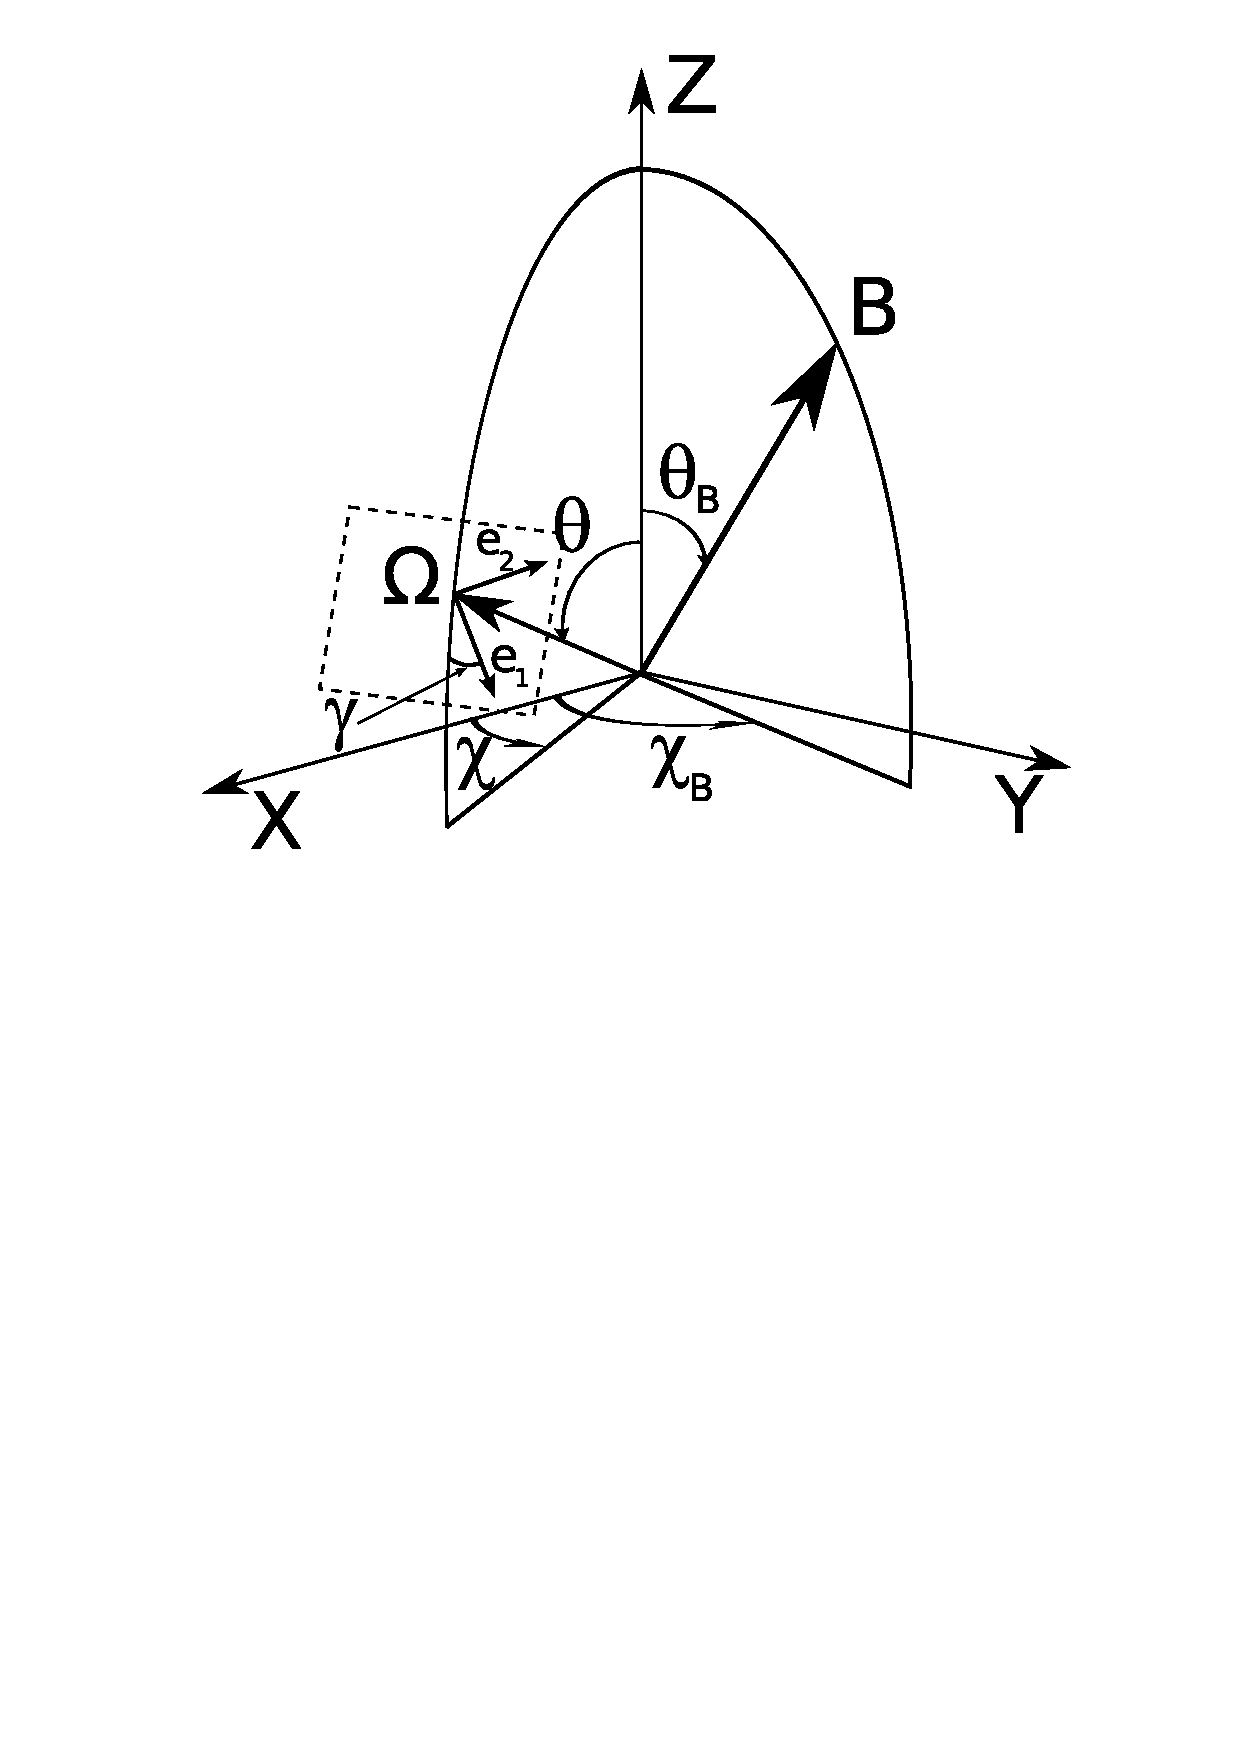
\includegraphics[width=0.4\textwidth]{f1.pdf}
\includegraphics[width=0.5\textwidth]{fig2a.pdf}
\caption{Left) Hazel reference system, rigth) diagram indicating the position of the LOS vector.}
\label{fig:figure1}
\end{figure}


As we can see in Fig. \ref{fig:figure1}, the angle $\chi$ is measured from $X$ to $Y$, and $\theta$ is measured from $Z$ to $\Omega$. We can choose the angle $\chi$ in order to simplify the equations. If we choose $\chi= 0$, then $\Omega$ is between $Z$ and $X$. This configuration only happens when $X$ is radial and  points towards the disk center (DC). However, if we choose $\chi= 180$, then $\Omega$ is between $Z$ and $-X$. This configuration only happens when $X$ is radial and  points away from the disk center (DC). In the rigth panel we see where is $\Omega$ if we choose the value of $\chi$. 

The consecuences of choosing one option are: the reference system itself and the equations to find all the posible solutions.

\clearpage
\section{Example 1.}
We have the following data from our observation and we choose $\chi=$180d:
\begin{itemize}
\item Position [arcsec]: $x=-300.0$; $y=-200.0$ \& Q$>$0: N-S
\end{itemize}

We can calculate the angle from the equator:
\begin{lstlisting}
alpha = np.arctan(y/x)*180./(np.pi) = 33.7d
\end{lstlisting}
Then we can calculate the heliocentric angle:
\begin{lstlisting}
theta = np.arcsin(np.sqrt(x**2.+y**2.)/960.)*180/np.pi = 22.1d
\end{lstlisting}
Now we can calculate $\gamma$ (must be measured from X to Y, anticlockwise). In Fig. \ref{fig:example1} (right) you have two solutions: the purple and the blue one:
\begin{lstlisting}
Gamma(purple) = 360-(90+33.7)=236.3d    or     Gamma(blue) =(90-33.7) = 56.3
\end{lstlisting}
Q$>$0 is a line, not  a direction. Gamma is defined [0,180º] (look the Hazel GUI) so in principle you can choose the direction of Q$>$0 which makes Gamma  inside the range. In order to check the result, you can execute the 3D plot to visualize the result (Fig. \ref{fig:example1}).

\begin{figure}[ht!]
\centering
\includegraphics[width=0.35\textwidth]{example1A.pdf}
\includegraphics[width=0.55\textwidth]{example1B.pdf}
\includegraphics[width=0.55\textwidth]{example1_3D.pdf}
\caption{Hazel reference system}
\label{fig:example1}
\end{figure}
\clearpage
Then, the angles for this observation are:
\begin{lstlisting}
theta_OBS = 22.1d
chi_OBS = 180.0d
Gamma_OBS =(90-33.7) = 56.3
\end{lstlisting}


\section{Example 2.}
We have the same observation but we choose $\chi=$0d. Now, $\gamma$ is again measured from $X$, and it is the same as before (Fig. \ref{fig:example2}).
\begin{lstlisting}
Gamma(blue) =(90-33.7) = 56.3
\end{lstlisting}

\begin{figure}[ht!]
\centering
\includegraphics[width=0.35\textwidth]{example2A.pdf}
\includegraphics[width=0.55\textwidth]{example2B.pdf}
\includegraphics[width=0.55\textwidth]{example2_3D.pdf}
\caption{Hazel reference system}
\label{fig:example2}
\end{figure}


Then, the angles for this observation are:
\begin{lstlisting}
theta_OBS = 22.1d
chi_OBS = 0.0d
Gamma_OBS =(90-33.7) = 56.3
\end{lstlisting}





\end{document}
